%%%%%%%% ICML submission — PDM2 %%%%%%%%%%%%%%%%%
% Built against icml2026.sty; swap for icml2027.sty when ICML 2027 publishes it
% (the macros used here have been stable across editions).

\documentclass{article}

\usepackage{microtype}
\usepackage{graphicx}
\usepackage{subcaption}
\usepackage{booktabs}
\usepackage{hyperref}

\newcommand{\theHalgorithm}{\arabic{algorithm}}

\usepackage{icml2026}

\usepackage{amsmath}
\usepackage{amssymb}
\usepackage{mathtools}
\usepackage[capitalize,noabbrev]{cleveref}
\usepackage{amsthm}
\newtheorem{definition}{Definition}

\icmltitlerunning{When Does Encoding Dynamics as Colour Help?}

\begin{document}

\twocolumn[
\icmltitle{When Does Encoding Dynamics as Colour Help?\\
           Seven Handwriting Cohorts and an Acquisition Floor}

\icmlsetsymbol{equal}{*}

\begin{icmlauthorlist}
\icmlauthor{Anonymous}{anon}
\end{icmlauthorlist}

\icmlaffiliation{anon}{Anonymous Institution}

\icmlcorrespondingauthor{Anonymous}{anon@example.com}

\icmlkeywords{time series to image, representation learning, shortcut learning,
              benchmark validity, handwriting}

\vskip 0.3in
]

\printAffiliationsAndNotice{}

\begin{abstract}
A recurring recipe turns a sampled trajectory into an image and hands it to a vision model:
the path is drawn as ink, and a per-sample signal --- speed, pressure, pen tilt --- is painted
along it as colour. The recipe is cheap, it reuses pretrained vision backbones, and it has been
reported to work. It is much less clear \emph{when} it works, or how much of a reported gain is
the encoding at all.

We run one pipeline, unchanged, across seven handwriting cohorts: five clinical and two
non-clinical, from a stylus on a graphics tablet to a bare finger on a phone screen. The encoding
gains $+0.17$ to $+0.25$ macro F1 over the bare trace in the two cohorts where the task dictates
the figure and only the execution differs, and nothing ($\left|\Delta\right| \leq 0.015$) in the
three where the produced shape carries the label in all or most tasks. The one cohort built to
hold both regimes in quantity falls between them, at $+0.05$. A control that displaces the signal
along the trace while preserving its distribution returns the texture-descriptor score to its
bare-trace baseline wherever that descriptor gains, and costs nothing where it does not. The controlled version of the test --- a directional
hypothesis registered before the splits were drawn, inside that mixed cohort, with the same
children, tablet and session on both sides --- came out backwards, and we report it as a failure of
the rule rather than re-describing it.

The second result was not by design. In three of these cohorts a classifier given two numbers that
contain no handwriting at all --- the median sampling interval and the session clock origin ---
matches or beats every pipeline we ran. It reaches $0.97$ inside one release of a widely used
benchmark, which forced us to discard those recordings, and $0.93$ on a second, where it beats
every real arm. The level of a score on such a benchmark is therefore not evidence that handwriting
was measured. We argue that the quantity carrying evidence is the margin over this acquisition
floor, give the ten-line procedure that measures it, and report it for every cohort with a
participant endpoint. That includes the cohort whose registered test failed, where six acquisition
descriptors predict the label better than any image or kinematic pipeline we ran --- which bounds
how far that failure can be read as evidence about pen dynamics.
\end{abstract}

\section{Introduction}
\label{sec:intro}

Converting a time series to an image and classifying the image with a convolutional network is an
old idea with a steady stream of new instances. In the handwriting literature the specific form is
appealingly direct: the pen path is already two-dimensional, so it can be drawn as it was written,
and whatever else the digitiser recorded at each sample --- speed, pressure, azimuth, altitude ---
can be mapped onto the colour of the stroke at that point. The result is an image in which
\emph{where} a dynamic quantity occurred along the trace is preserved rather than aggregated away,
which is exactly the information that a vector of summary statistics discards. We call such an
image a \emph{pseudodynamic minimap}, following the formulation of
\citet{prior2027minimaps}, whose single-cohort result this paper sets out to transfer and test.

The appeal is obvious; the evidence is thinner than it looks. Published results are typically a
single cohort, a single acquisition device, and a comparison against a baseline chosen by the same
authors. That leaves two questions unanswered, and this paper is about both.

\paragraph{When does the encoding help?} An encoding that adds a channel cannot hurt in principle,
but it can in practice: it spends model capacity, it changes the texture statistics a descriptor
sees, and it can only pay for itself if the added channel carries information the shape does not.
We state that condition sharply and test it.

\paragraph{How would you know?} Clinical handwriting corpora are assembled over months, often with
patients and controls recruited through different routes and recorded in different sessions. Any
quantity that drifts with the session --- the digitiser's sampling rate, the moment the clock
started --- is then correlated with the label without passing through the disease. This is not a
hypothetical, and \cref{sec:floor} measures how far it goes.

\paragraph{Contributions.}
\begin{itemize}
\itemsep0em
\item \textbf{A transfer study with one pipeline.} Seven cohorts, identical rendering parameters,
descriptor, model grid, nested protocol and statistics; every design decision for every cohort
registered in a protocol document before any metric was computed
(\cref{sec:cohorts,sec:protocol}).

\item \textbf{A candidate rule, tested in both directions, and one failure reported as such.} The
minimap helps when the label is not in the shape, and not otherwise. Across cohorts this separates
the two gains from the three nulls, and the one cohort built to hold both regimes falls between
them. \emph{Within} that cohort --- same children, tablet and session on both sides --- a
hypothesis registered with its direction before the splits were drawn is \textbf{not} confirmed:
the margin is larger on the half where the rule predicts none. We report the failure, and we use the floor of the next contribution to bound
what it can mean (\cref{sec:when}).

\item \textbf{A mechanism control.} Circularly shifting the signal along each stroke, and
permuting it within each stroke, leave every marginal intact and destroy only \emph{where} the
signal sits. Run with the texture descriptor on the six cohorts that have a participant endpoint,
its cost tracks that descriptor's gain; it has not yet been run with the CNN descriptor
(\cref{sec:when}).

\item \textbf{The acquisition floor.} A two-feature classifier containing no handwriting reaches
$0.97$ inside one public clinical benchmark and $0.93$ on a second, where it beats every real arm;
on a third it matches four real pipelines including our own. We define the floor, give the
procedure, and report every result of the main table as a margin over it
(\cref{sec:floor,sec:results}).
\end{itemize}

We are explicit about what the floor result is not. It is not a claim that published models read
the clock: our renderers never see an absolute timestamp. It is a claim about what a number means.
A macro F1 of $0.93$ on a benchmark whose floor is $0.93$ is consistent with having measured
nothing about handwriting, and the reader of such a paper currently has no way to tell.

\section{Related work}
\label{sec:related}

\paragraph{Time series as images.} Encoding a sequence as a picture so that an image model can be
applied to it spans recurrence plots \citep{eckmann1987recurrence}, Gramian angular fields and
Markov transition fields \citep{wang2015gaf}, and more recently direct rasterisations of
trajectories. What distinguishes the handwriting case is that the
series already has a faithful two-dimensional embedding, so the encoding does not have to invent a
geometry: the question is only what to do with the remaining channels.

\paragraph{Handwriting as a clinical signal.} Digitised handwriting has been used as a marker for
Parkinson's disease and for developmental dysgraphia, and as a marker of cognitive decline
\citep{werner2006handwriting}. The dominant
representation is a vector of kinematic and pressure statistics
\citep{drotar2016pahaw,drotar2020dysgraphia}; image-based alternatives are more recent. Our
baselines include both.

\paragraph{Shortcut learning and benchmark validity.} That models latch onto acquisition artefacts
rather than the phenomenon is well documented \citep{geirhos2020shortcut}, and in medical imaging
in particular, where scanner and site identity leak into diagnostic labels
\citep{degrave2021shortcut}. The contribution we make here is not the observation but the
instrument: a floor that is cheap enough to report with every result, and that we show is not a
corner case in this domain.

\section{Pseudodynamic minimaps}
\label{sec:method}

A recording is a sequence of samples $p_i = (x_i, y_i, t_i, c_i, \mathbf{s}_i)$, with position,
timestamp, a contact flag and a vector of per-sample signals. Only segments with contact at both
ends are drawn.

\paragraph{Geometry.} Contact points are fitted to a $512 \times 512$ canvas with a $20$~px margin,
preserving aspect ratio, and drawn as $4$~px line segments with $3\times$ supersampling followed by
Lanczos downsampling. We also report a second geometry in which the scale is fixed per task in
device units rather than fitted per recording, so that absolute size is preserved across
participants.

\paragraph{Colour.} For a chosen signal $s$ and segment $i$, the value is the mean of its endpoints,
$\bar{s}_i = (s_i + s_{i+1})/2$, normalised \emph{within the recording} by its own $5$th and $95$th
percentiles,
\begin{equation}
\tilde{s}_i = \mathrm{clip}\!\left(\frac{\bar{s}_i - q_{05}(s)}{q_{95}(s) - q_{05}(s)},\, 0,\, 1\right),
\end{equation}
and mapped affinely to a channel range $[30, 220]$. Speed is $\log(1+v)$ before normalisation;
azimuth is centred circularly before normalisation. Three signals can be assigned to the three
channels at once, giving the nine encodings we evaluate: the bare trace, four single-signal
minimaps (\textbf{S}peed, \textbf{P}ressure, \textbf{A}ltitude, a\textbf{Z}imuth) and four triples.

\begin{figure}[t]
\begin{center}
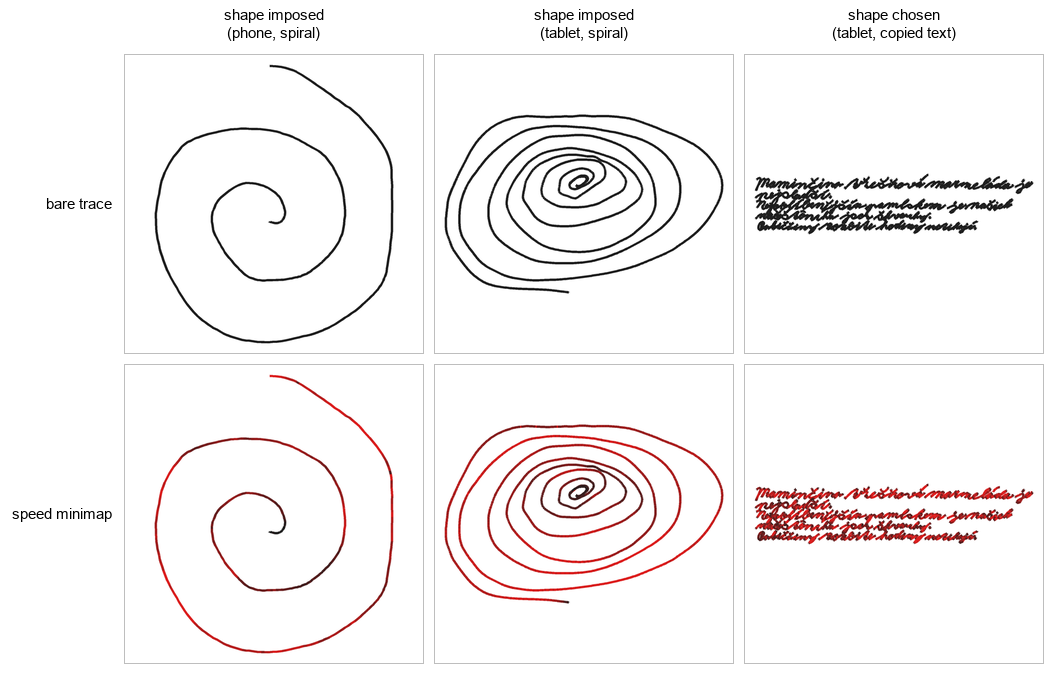
\includegraphics[width=\columnwidth]{figures/examples.png}
\end{center}
\caption{The same encoding on the two regimes of \cref{sec:when}, read from recordings the
experiments actually used. Left and centre: the task prescribes the figure, so the bare trace is
nearly the same for everyone and what differs is the execution the colour carries. Right: a copied
text, where the produced shape already carries most of what distinguishes one recording from
another --- and where the square canvas, fixed for every cohort, shrinks a wide multi-line page
into a strip. No participant is identified and no panel was chosen for its appearance.}
\label{fig:examples}
\end{figure}

Two properties matter for the argument. The normalisation uses no statistic of the cohort and no
label, so nothing about the class distribution can enter the image. And the mapping is
\emph{positional}: it is the only part of the pipeline that records where along the trace a value
occurred, which is what \cref{sec:when} tests directly.

\paragraph{Descriptor and model.} Unless stated otherwise, images are described by Local Phase
Quantisation \citep{ojansivu2008lpq} on each channel ($64 \times 64$, $5\times 5$ window, $256$ bins per channel, $768$
dimensions, square-root transformed) and classified by a support vector machine. We also report a
frozen ImageNet ResNet18 \citep{he2016resnet} as a second descriptor over the identical images, with an
$\ell_2$-regularised logistic head, to separate the contribution of the encoding from that of the
descriptor.

\section{Evaluation protocol}
\label{sec:protocol}

Every cohort is evaluated identically, and every decision --- inclusion rule, task definition,
contact rule, unit conversion, split design --- was written into a per-cohort protocol document
\emph{before} any classifier was fitted on that cohort. Where the direction of the study changed
mid-stream, the protocol carries a dated addendum rather than a rewrite.

\paragraph{Partitions.} Five repeats of five stratified outer folds, three inner folds for
selection, nested so that representation and hyperparameters are chosen on training participants
only. \textbf{The participant is the unit}: all recordings of a participant are in the same fold,
and participant decisions are the majority vote over the available tasks. Screening and
confirmation use disjoint master seeds; we treat split-to-split variation of $\pm 0.03$ macro F1 as
noise, and report no gain that does not reappear on the confirmation seed.

\paragraph{Statistics.} Confidence intervals are $10{,}000$ label-stratified participant bootstrap
resamples. Paired contrasts use participant-wise swap randomisation. Multiplicity is corrected by
the Holm procedure \citep{holm1979} within families declared in the protocol.

\paragraph{Spatial controls.} To test whether a gain comes from \emph{where} the signal sits, we
apply two destructive controls at render time, each preserving every per-stroke marginal exactly:
a \emph{circular shift} of the signal values along each stroke, and a \emph{joint permutation} of
the signal values within each stroke. Both leave the ink identical and the colour histogram
identical; only the correspondence between position and value is destroyed.

\section{The acquisition floor}
\label{sec:floor}

\begin{definition}[Acquisition floor]
For a cohort $\mathcal{D}$ and an evaluation protocol $\Pi$, the acquisition floor
$\phi(\mathcal{D}, \Pi)$ is the score that $\Pi$ assigns to a classifier whose only inputs are
properties of the recording process that no behaviour of the subject can produce.
\end{definition}

We instantiate it with two features per recording: the \textbf{median sampling interval between
consecutive contact samples}, and $\log_{10}$ of the \textbf{first timestamp}, that is, the origin
of the session clock. Neither is a symptom. No disease makes a digitiser sample at $9$~ms instead
of $7$~ms, and none sets the clock. The second feature is independent of the writer by
construction. The first is only approximately so --- a digitiser can drop samples under fast
motion --- which is one reason to keep the probe to features whose dependence on behaviour is this
weak, and to report wider probes separately.

The floor is not chance. Chance is a property of the label distribution; the floor is a property of
the dataset as assembled, and it is the level below which a score is uninformative about the
phenomenon. We therefore report, for every arm and every cohort, the margin
$\Delta_\phi = \text{score} - \phi$, and treat $\Delta_\phi$ rather than the score as the quantity
that carries evidence.

Measuring it costs nothing: it reuses the protocol already in place, and the features are two
reductions over a timestamp column. We report it for all six cohorts that have a participant
endpoint, including those where our own results are positive; the signature cohort has neither
(\cref{sec:results}).

\section{Cohorts}
\label{sec:cohorts}

\begin{table}[t]
\caption{The cohorts analysed. \emph{Shape} is whether the produced figure carries the label, which \cref{sec:when} argues is what decides the outcome. \emph{Units} are participants and the parenthesis gives the class split, except in the two non-clinical cohorts, where the unit is the recording: Character Trajectories has a single writer, and in SVC2004 each of the $40$ writers contributes both classes, so a writer is not a class. $^{\dagger}$ParkinsonHW is reported on the only sub-cohort its own acquisition artefact leaves usable (36 patients from the second release plus the 15 controls, out of 76 participants in the full release); \cref{sec:floor} explains why.}
\label{tab:cohorts}
\vskip 0.1in
\begin{center}
\begin{small}
\begin{tabular}{llllrr}
\toprule
cohort & instrument & channels & shape & units & recordings \\
\midrule
ParkinsonHW$^{\dagger}$ & stylus, tablet & x, y, p, grip & fixed by task & 51 (15 / 36) & 98 \\
Zhu et al. & finger, phone & x, y only & fixed by task & 58 (30 / 28) & 116 \\
DiaGraMo & stylus, Cintiq & full & both & 273 (156 / 117) & 3796 \\
Drot\'ar--Dobe\v{s} & stylus, tablet & full & chosen by writer & 120 (57 / 63) & 120 \\
PaHaW & stylus, tablet & full & mixed & 75 (38 / 37) & 597 \\
Char.\ Trajectories & stylus, tablet & x, y, force & \textbf{is} the label & 853 (397 / 456) & 853 \\
SVC2004 & stylus, tablet & full & copied by forger & 1600 (800 / 800) & 1600 \\
\bottomrule
\end{tabular}
\end{small}
\end{center}
\vskip -0.1in
\end{table}


Seven cohorts, chosen to vary the instrument, the population and --- critically --- whether the
produced shape carries the label.

\paragraph{Shape fixed by the task.} In \textsc{ParkinsonHW} \citep{isenkul2014parkinsonhw} and
\textsc{Zhu} \citep{zhu2025smartphone} participants trace a
prescribed spiral or wave, so what differs between a patient and a control is execution, not
figure. \textsc{Zhu} is the extreme case of instrument change: a bare finger on a phone screen,
with no pressure and no angles, so the only minimap available is speed.

\paragraph{Shape chosen by the writer.} In \textsc{Drot\'ar--Dobe\v{s}}
\citep{drotar2020dysgraphia} and in the writing tasks of \textsc{DiaGraMo}
\citep{zvoncakova2026diagramo}, children write text; the produced shape varies with what was written.

\paragraph{Both, under one setup.} \textsc{DiaGraMo} is the pivot of the study. The same children,
the same tablet and the same session produce ten graphomotor tasks whose target figure is imposed
and four writing tasks whose shape is not, which lets the rule of \cref{sec:when} be tested without
changing anything else. It is the only cohort here that permits a controlled test of the rule, and
it is the cohort in which the rule fails.

\paragraph{Non-clinical controls.} \textsc{SVC2004} \citep{yeung2004svc} is signature
verification: a skilled forger
copies the shape deliberately, so the shape is uninformative by construction and only dynamics
remain --- the cleanest positive control in this set. \textsc{Character Trajectories} \citep{williams2006chartraj} is
its mirror image: the label \emph{is} the shape, since a reader identifies a character from ink alone.

\paragraph{Reference cohort.} \textsc{PaHaW} \citep{drotar2016pahaw} is the corpus on which the
encoding was originally reported \citep{prior2027minimaps}, and is included unchanged as a regression control.

\section{Results}
\label{sec:results}

\begin{table}[t]
\caption{Macro F1 at the unit level on the confirmation splits, which no model or encoding choice ever saw. $\Delta$ is the gain of the best minimap arm over the static trace; \emph{kinem.} is the 83 kinematic and pressure attributes computed from the same signals; \emph{floor} is the two-number acquisition classifier of \cref{sec:floor}, which contains no handwriting at all. $\Delta_\phi$, the margin over that floor, is the quantity that carries evidence: the score alone does not.}
\label{tab:headline}
\vskip 0.1in
\begin{center}
\begin{small}
\begin{tabular}{lrrrrrr}
\toprule
cohort & static & minimap & $\Delta$ & kinem. & floor & $\Delta_\phi$ \\
\midrule
ParkinsonHW$^{\dagger}$ & 0.757 & 0.925 & $+0.168$ & 0.854 & 0.666 & $+0.259$ \\
Zhu et al. & 0.627 & 0.879 & $+0.252$ & 0.843 & 0.473 & $+0.406$ \\
DiaGraMo & 0.658 & 0.708 & $+0.050$ & 0.716 & 0.453 & $+0.256$ \\
Drot\'ar--Dobe\v{s} & 0.767 & 0.777 & $+0.010$ & 0.783 & 0.929 & $-0.152$ \\
PaHaW & 0.634 & 0.636 & $+0.002$ & 0.650 & 0.642 & $-0.006$ \\
Char.\ Trajectories & 0.982 & 0.996 & $+0.015$ & 0.998 & 0.501 & $+0.495$ \\
\bottomrule
\end{tabular}
\end{small}
\end{center}
\vskip -0.1in
\end{table}


\cref{tab:headline} is to be read from the right. The score column says how a cohort behaves; the
$\Delta_\phi$ column says whether the behaviour is about handwriting.

\paragraph{Where the encoding gains, it gains a lot.} On the two cohorts in which the task dictates
the figure, the best minimap arm beats the bare trace by $+0.252$ (\textsc{Zhu}, $0.627 \to 0.879$)
and $+0.168$ (\textsc{ParkinsonHW}, $0.757 \to 0.925$). Both sit far above their own floors
($\Delta_\phi = +0.406$ and $+0.259$), both exceed the $83$ kinematic and pressure attributes
computed from the identical signals, and both reproduce on the confirmation seed. Because the two
differ in almost everything --- a stylus on a graphics tablet against a bare finger on a phone
screen, with no pressure and no pen angles available in the second --- the gain is not a property of
one digitiser.

The gains are also large relative to what is left to gain. Above a static-trace baseline of $0.627$
and $0.757$ there is $0.373$ and $0.243$ of headroom; the minimap captures $68\%$ and $69\%$ of it.
We give this comparison only for these two cohorts, where the baseline leaves room for it to mean
something.

\paragraph{Where the shape carries the label, the encoding does nothing.} On
\textsc{Drot\'ar--Dobe\v{s}} the margin is $+0.010$, on \textsc{PaHaW} $+0.002$, and on
\textsc{Character Trajectories} $+0.015$ --- all inside the $\pm 0.03$ band we declared as split
noise. Only the character null was registered in advance as a directional hypothesis; the other
two were not. The character cohort is the sharpest of
the three because every arm is above $0.98$: a reader identifies a character from ink alone, so
there is nothing for dynamics to add. We restored headroom there without choosing a task after
seeing a metric, by running the canonical $20$-class problem over all $2{,}858$ recordings instead
of the three declared pairs (Addendum~A of its protocol). The static trace reaches $0.944$ and the
best minimap $0.956$: a margin of $+0.012$, positive in $23$ of the $25$ outer folds (Wilcoxon
$p = 3 \times 10^{-7}$) and an order of magnitude below the Parkinson cohorts. A real effect, and a
negligible one.

%% Generated by scripts/x3_paper_tables.py from runs/. Do not edit by hand.
%% Every number below comes from the run that produced it. An edit here is silently overwritten
%% the next time the generator runs, and breaks the guarantee that no number in the paper can
%% differ from its run. To change a number, change the run or the generator.
\begin{table}[t]
\caption{SVC2004 skilled-forgery verification, writer-independent, single held-out split. Reported apart from \cref{tab:headline} because this cohort has no participant endpoint and no acquisition floor: a forger and a genuine signer are not two groups of people. It is the cleanest case of a label the shape cannot carry, since the forgery copies the shape on purpose, and the static trace sits at chance while every encoding that carries a signal scores above it. A single split carries no interval, so the smallest of those margins should not be read as established.}
\label{tab:signature}
\vskip 0.1in
\begin{center}
\begin{small}
\begin{tabular}{lrrr}
\toprule
encoding & macro F1 & accuracy & ROC AUC \\
\midrule
static & 0.491 & 0.492 & 0.505 \\
S & 0.528 & 0.531 & 0.543 \\
P & 0.564 & 0.567 & 0.586 \\
A & 0.533 & 0.534 & 0.555 \\
Z & 0.533 & 0.534 & 0.557 \\
SPA & 0.581 & 0.583 & 0.617 \\
SPZ & 0.589 & 0.593 & 0.631 \\
SAZ & 0.576 & 0.580 & 0.618 \\
PAZ & 0.613 & 0.617 & 0.653 \\
\bottomrule
\end{tabular}
\end{small}
\end{center}
\vskip -0.1in
\end{table}


\paragraph{The positive control behaves as the rule predicts.} \textsc{SVC2004}
(\cref{tab:signature}) is the limiting case: a skilled forger copies the shape on purpose, so the
shape is uninformative by construction. The static trace is at chance ($0.491$ macro F1, ROC AUC
$0.505$) and every encoding carrying a signal scores above it, from $0.528$ for speed alone up to
$0.613$ and $0.653$ for the pressure--altitude--azimuth triple. We report it apart from \cref{tab:headline} because it has
neither a participant endpoint nor a floor --- a forger and a genuine signer are not two groups of
people --- so it is evidence about the rule and not about clinical performance.

\paragraph{On two cohorts the floor swallows the result.} \textsc{Drot\'ar--Dobe\v{s}} scores
$0.777$ with the minimap and $0.783$ with the kinematic attributes, and $0.929$ with two numbers
that contain no handwriting: $\Delta_\phi = -0.152$. Every pipeline we ran on that cohort is worse
than its clock. On \textsc{PaHaW} the floor is $0.642$ against $0.636$ and $0.630$ for the LPQ and
ResNet18 minimaps, $0.650$ for the kinematic attributes and $0.634$ for the bare trace: four
pipelines and an artefact, indistinguishable.
\textsc{ParkinsonHW} is the case that forced us to define the floor at all. Inside its
\texttt{hw\_dataset} release the two features reach $0.973$, because the digitiser's sampling period
separates those patients from everything else; the sub-cohort that remains once they are removed
($36$ patients and $15$ controls) is the one reported here, and on it the minimap keeps a margin of
$+0.259$ over the floor. The artefact therefore does not explain that cohort's gain --- but without
measuring it we could not have known, and a result reported on the whole release would be computed
partly on recordings that a two-number classifier separates at $0.973$.

\paragraph{A narrow floor is not a clean cohort.} The two-feature probe is deliberately minimal,
and widening it slightly changes the picture twice. Adding sample count, duration and the mean and
standard deviation of the contact interval --- six acquisition descriptors, none of them a property
of the writing ---
reaches $0.784$ on \textsc{DiaGraMo}, above every image arm and above the kinematic attributes
($0.716$), and $1.000$ on \textsc{Character Trajectories}, where the narrow floor is exactly
$0.501$. The character case is instructive rather than alarming: duration and sample count encode
how long a character takes to write, which legitimately identifies it. That is the reason we keep
the floor narrow enough that no behaviour of the writer can move it, and report the six-feature arm
separately as an upper bound rather than as a floor.

\section{When the encoding helps}
\label{sec:when}

\paragraph{The rule.} The pattern in \cref{tab:headline} separates the cohorts into two groups: the
minimap gains where the produced figure is imposed by the task and the label lives in the execution
($+0.168$ and $+0.252$), and gains nothing where the produced shape itself carries the label
($+0.010$, $+0.002$, $+0.015$). \textsc{PaHaW} sits in the second group because seven of its eight
tasks are writing, although the first is a spiral; its null is also level with its floor, so it
weighs little either way. \textsc{DiaGraMo}, whose fourteen task slots mix the two regimes,
falls between the groups at $+0.050$; it is consistent with the ordering and it is the one cohort
that belongs cleanly to neither group. The signature cohort extends the rule to a non-clinical
label, and the character cohort anchors its null end. This is a regularity over seven datasets,
stronger than the single-cohort evidence the recipe is usually reported with and weaker than a
controlled test: acquisition, population and task change together between cohorts.

\begin{table}[t]
\caption{Spatial controls on the LPQ selection arm, screening splits. Both destroy only the correspondence between position along the stroke and signal value, leaving the ink, the contact mask and every per-stroke marginal identical. A cost means the classifier reads \emph{where} the signal sits along the trace; no cost means it reads only how the values are distributed.}
\label{tab:controls}
\vskip 0.1in
\begin{center}
\begin{small}
\begin{tabular}{lrrrrr}
\toprule
cohort & minimap & shift & permuted & $\delta$ shift & $\delta$ perm. \\
\midrule
ParkinsonHW$^{\dagger}$ & 0.738 & 0.637 & 0.624 & $-0.101$ & $-0.114$ \\
Zhu et al. & 0.750 & 0.688 & 0.649 & $-0.062$ & $-0.101$ \\
DiaGraMo & 0.645 & 0.669 & 0.648 & $+0.024$ & $+0.003$ \\
Drot\'ar--Dobe\v{s} & 0.783 & 0.758 & 0.772 & $-0.025$ & $-0.011$ \\
PaHaW & 0.590 & 0.586 & 0.607 & $-0.004$ & $+0.017$ \\
Char.\ Trajectories & 0.989 & 0.985 & 0.989 & $-0.004$ & $+0.000$ \\
\bottomrule
\end{tabular}
\end{small}
\end{center}
\vskip -0.1in
\end{table}


\paragraph{The gain is positional.} \cref{tab:controls} removes the one thing the encoding adds.
Both controls keep the ink, the contact mask and every per-stroke colour marginal identical, and
destroy only the correspondence between position along the stroke and signal value. Every column of
the table comes from the same run, so each row can be read against its own static baseline. Where
there is a gain, both controls return the score to that baseline: on \textsc{ParkinsonHW} a
$+0.098$ gain over $0.640$ falls back to $0.637$ and $0.624$, and on \textsc{Zhu} a $+0.067$ gain
over $0.683$ falls back to $0.688$ and $0.649$. Where there is no gain there is nothing to remove,
and the controls move the score by less than the noise band in either direction --- on
\textsc{DiaGraMo} the shift is nominally \emph{better} than the authentic images. So the LPQ gain,
where it exists, comes from \emph{where} along the trace a value occurred and not from the
distribution of values, which is the only thing a minimap encodes that a summary vector does not.
The larger ResNet18 gains of \cref{tab:headline} have been put through the same controls on
\textsc{DiaGraMo}, reported below; on the two cohorts that carry the cross-cohort gain they have
not.

\paragraph{A channel that contains nothing.} The two controls above move the real values along the
stroke, so neither can tell whether a gain comes from what the channel contains or from the act of
adding a channel that varies at all --- both conditions still paint the real signal. We therefore
paint channels that carry no information about the writer and change nothing else: the acquisition
index as a ramp, an AR(1) sequence whose lag-1 autocorrelation is taken from that recording's own
signal so that its smoothness matches, and white noise. The nulls are written into the signal column
the renderer passes through untransformed, so they receive the identical normalisation and
rasterisation; the direction was registered before the run, with the threshold at which we would
have concluded that the encoding's benefit is the channel addition rather than its content.

On \textsc{Zhu}, which carries the largest reported gain in the study and has one dynamic signal so
that no selection enters the comparison, the control passes under LPQ. The real speed channel gains
$+0.109$ over the static trace (CI $+0.036$ to $+0.189$); the three nulls gain $+0.029$, $-0.015$
and $-0.012$, every interval across zero. The $+0.029$ is the ramp, the null we declared weakest
because it still encodes how the trace was parameterised in time, and we report it at the edge of
the band rather than inside it. Under the frozen backbone the same question has no content, because
that descriptor has no encoding gain here to explain: the bare trace reaches $0.893$ and the real
minimap $0.879$, with every null in the same place. What a minimap paints matters to the local
descriptor and not to the backbone, on this cohort.

\begin{table*}[t]
\caption{The contrast inside DiaGraMo: the same children, the same tablet, the same session. Ten tasks impose the target figure, four do not, and the direction was registered before the splits were drawn. It came out backwards, and the \emph{nuisance} column --- six acquisition descriptors, no handwriting in them --- shows why that outcome cannot be read as evidence about pen dynamics.}
\label{tab:diagramo}
\vskip 0.1in
\begin{center}
\begin{small}
\begin{tabular}{lrrrrrr}
\toprule
task set & static & LPQ & ResNet18 & $\Delta$ best & floor & nuisance \\
\midrule
all 14 tasks & 0.658 & 0.637 & 0.708 & $+0.050$ & 0.453 & 0.784 \\
graphomotor (10) & 0.616 & 0.599 & 0.647 & $+0.030$ & 0.432 & 0.593 \\
writing (4) & 0.635 & 0.623 & 0.703 & $+0.069$ & 0.424 & 0.846 \\
\bottomrule
\end{tabular}
\end{small}
\end{center}
\vskip -0.1in
\end{table*}


\paragraph{The within-cohort test, and its failure.} The cross-cohort rule invites one controlled
experiment, and \textsc{DiaGraMo} supplies it: $273$ children, one tablet, one session,
$3{,}796$ recordings, of which ten task slots impose the target figure (spirals, loops, a saw, a
rainbow) and four do not (dictation, free recall, copy). We registered the direction before drawing
the splits: the minimap margin should be larger on the graphomotor slots than on the writing slots
(H1), and within noise of zero on the writing slots (H2).

Both fail, and in the same direction. On the confirmation splits the margin is $+0.030$ on the
graphomotor slots ($95\%$ CI $-0.009$ to $+0.070$, $p_{\text{Holm}} = 1.00$) and $+0.069$ on the
writing slots (CI $+0.020$ to $+0.119$, $p_{\text{Holm}} = 0.036$). The predicted ordering is
reversed, and only the writing slots --- the half where the rule says the encoding should be
useless --- clear the noise band. The screening splits agree ($+0.026$ against $+0.079$), so this is
not one unlucky partition. We report this as a failure of the rule in the one place we could test
it without changing anything else, and we have not re-worded the rule to accommodate it.

\paragraph{What the failure is, and what it is not.} Two measurements bound how much the failure
can be read as evidence about pen dynamics, and both point the same way.

First, the entire margin on the writing slots comes from the frozen ResNet18 arm. The LPQ arm --- the
descriptor the method was defined with --- sits at or below the static trace in every
\textsc{DiaGraMo} task set ($-0.021$ on all $14$, $-0.018$ on graphomotor, $-0.012$ on writing).
Putting the two spatial controls through the frozen backbone instead, which this section previously
named as the experiment we were missing, shows why. The test needs a static trace described by the
same backbone, an arm the pipeline did not have; against that baseline the encoding adds nothing in
this cohort, in any task set: $0.726$ static against $0.719$ minimap on the writing slots, $0.672$
against $0.660$ on graphomotor and $0.714$ against $0.708$ on all $14$, every contrast a null on
screening splits. The $+0.069$ margin is thus the difference between two descriptors over the same
images rather than between two encodings under one descriptor, and within the descriptor there is no
margin for a control to remove. The controls behave accordingly: on the writing slots they cost
$+0.020$ and $+0.002$, both inside the noise band and both intervals across zero. Their direction
and a threshold of $+0.03$ were registered as H4 before the run, against the alternative H5 that
they would cost nothing because neither control changes how much a child wrote; H4 fails and H5 is
weakly supported, as the addendum said in advance it could only be.

Second, \cref{tab:diagramo} puts the acquisition arms beside the image arms, and the split falls
exactly where the hypothesis broke. The narrow floor is at chance in both halves ($0.432$ and
$0.424$), so no clock artefact is involved. But six descriptors of the recording process --- sample
count, duration and four timing statistics, none of them describing the ink --- reach
$\mathbf{0.846}$ on
the writing slots and only $0.593$ on the graphomotor slots. On the half where the registered
prediction failed, how much a child wrote and for how long predicts the label far better
($0.846$) than the best image arm ($0.703$) or the $83$ kinematic attributes ($0.789$); on the half
where the rule predicted a gain, the same descriptors are below the static trace.

That is the reading we find most likely. Multi-line dictation and copy vary enormously in
length between children, a single spiral does not, and a global CNN descriptor over a canvas-fitted
page is well placed to read quantity off the ink. We cannot separate that explanation from a
genuine dynamic effect with the experiments we have, and we do not claim to --- but a margin
obtained on a subset whose nuisance ceiling is $0.846$ is not evidence that the rule is wrong
either. The registered prediction failed; what replaced it is not a better claim about dynamics
but a measurement of why that subset could not have tested one.

\paragraph{The third hypothesis, and why it decides nothing.} H3 predicted that the spatial
controls would cost more on the graphomotor slots than on the writing slots. Per task set, the cost
of the circular shift is $-0.007$ and $-0.003$ and the cost of the permutation $+0.015$ and
$-0.012$: nominally in the predicted direction for the permutation and against it for the shift,
entirely inside the noise band, every interval across zero and every corrected $p$ equal to $1.00$. We registered that this would happen before
running it, for a stated reason: the controls are implemented for the LPQ arm, which has no gain on
this cohort, so there is nothing positional for them to destroy whichever half they run on. H3 is
reported as uninformative rather than as support.

\paragraph{What the backbone controls leave open.} The ResNet18 margin on \textsc{DiaGraMo} is no
longer untested, and the test dissolved the thing it was aimed at: there is no within-descriptor
margin on that cohort for a control to remove. The same question stays open where it matters more
for the rule. On \textsc{ParkinsonHW} and \textsc{Zhu} the headline margins are also ResNet18
margins, while the gains the controls act on are the LPQ ones, $+0.086$ and $+0.109$, which do fall
back to baseline when position is destroyed. A static trace described by the backbone on those two
cohorts needs no new rendering and is the first thing we would run next. Until it exists, the
cross-cohort rule rests on the arm where the controls locate the gain, and its one within-cohort
test neither confirmed it nor, given the nuisance ceiling above, cleanly refuted it.

\section{Conclusion}
\label{sec:conclusion}

One pipeline across seven cohorts supports a narrow claim: painting a per-sample signal along the
trace earns its place when the task fixes the figure and the label lives in the execution, and
earns nothing once the produced shape already carries the label. The mechanism control puts the
texture-descriptor gain where the encoding puts it, and the one experiment that holds cohort, device and session fixed
did not confirm the rule --- on the half where the rule predicts nothing, six acquisition
descriptors predict the label better than any image arm we ran, which is also why that half could
not have tested it. If one result here outlives the rest, we would prefer it to be the floor: two
features, no handwriting in them, and on two public benchmarks a score that nothing in this paper
beats. Reporting a margin over it costs a few lines and changes what a score means.

\section{Limitations}
\label{sec:limitations}

\paragraph{Cohort sizes.} Four of the seven cohorts have fewer than $130$ participants. Confidence
intervals are correspondingly wide and we report them everywhere rather than point estimates alone.

\paragraph{Two descriptors.} The conclusion that the encoding helps in a given regime is a
conclusion about these two descriptors over these images. We report both because they disagree in
magnitude, and the disagreement is itself informative.

\paragraph{The floor is a lower bound on leakage, not an audit.} Two features is a deliberately
small probe. A cohort whose floor is at chance is not thereby clean; it is only clean of the two
artefacts we measured.

\paragraph{Character Trajectories is a reconstruction.} Its released signals are differentiated,
smoothed and temporally aligned by the original authors, so it is reported as a directional control
rather than as a measurement of raw dynamics.

\paragraph{The headline margin adds a change of encoding to a change of descriptor.} $\Delta$ in
\cref{tab:headline} is the best minimap arm over the LPQ static trace, and on four of the six
cohorts with a participant endpoint the best minimap arm is the ResNet18 one. On the two cohorts
where a backbone static baseline now exists, that baseline removes the ResNet18 margin: on
\textsc{DiaGraMo} in all three task sets, and on \textsc{Zhu} on the confirmation splits, where the
bare trace under the backbone reaches $0.893$ against the minimap's $0.879$ and beats the LPQ
minimap by $+0.156$. \textsc{Zhu}'s $\Delta = +0.252$ is therefore the sum of an encoding gain of
$+0.109$, which the nulls and the spatial controls both localise, and a descriptor gain that the
definition attributes to the encoding. We report $\Delta$ as defined, state the decomposition where
we have measured it, and name the same baseline on \textsc{ParkinsonHW} as the measurement this
paper is missing.

\paragraph{The rule may be relative to the descriptor.} On \textsc{Zhu} the task fixes the figure,
so we took ``the label is not in the shape'' to hold. The backbone reads the label off the bare
trace at $0.893$, so for that descriptor the shape does carry it. Whether the antecedent of the
rule is a property of the task or of the descriptor is not something one cohort of $58$
participants decides, and we have not tested it; we state it because our own data raise it.

\paragraph{The mechanism control covers one descriptor and, on one cohort, both.} The spatial
controls are described with LPQ on every cohort and with the frozen backbone on \textsc{DiaGraMo}
only. Where the LPQ arm has no gain the controls have little to destroy, which is why
\cref{sec:when} reads the DiaGraMo nulls as weak evidence rather than as demonstrations.

\paragraph{SVC2004 is a single split.} It is evaluated writer-independently on one held-out
partition, without the nested repeats the other cohorts receive, and without a floor. It supports
the rule; it does not carry a confidence interval.

\paragraph{The two large gains come from cohorts of $51$ and $58$ participants.} Nothing
here is a sample size from which a clinical claim follows. The transfer result is about when an
encoding earns its place in a representation, not about screening for disease.

\section*{Impact Statement}

This paper evaluates representations for handwriting and reports that two public clinical
benchmarks are separable from acquisition metadata alone. We want to be precise about what
follows and what does not.

Nothing here shows that any published model used that metadata; the pipelines we and others run do
not see it. What it shows is that the \emph{level} of a score on these benchmarks is uninformative
on its own, and that the appropriate reference point is the cohort's own floor rather than chance.
We regard this as a reason to report the floor routinely, not a reason to discard the datasets or
to doubt the clinical phenomenon, which is well established by other means.

The application domain is diagnostic. We make no claim of clinical utility for any model in this
paper: the cohorts are small, the labels are study labels rather than screening outcomes, and the
margins we report are far from what a deployed decision would require.

\bibliography{main}
\bibliographystyle{icml2026}

\end{document}
